\documentclass{article}
\usepackage{KJN}
\usepackage{a4wide,changebar}
\usepackage[numbered,framed]{mcode}

\title{Introduction to Vision and Robotics: Assignment 1}
\author{Chris Swetenham: Student Num, Daniel Mankowitz: S1128165}
\date{3/11/2011}

\begin{document}
\maketitle

\section{Introduction}
\label{sec:introduction}
An overview of the main ideas used in the approach


\section{Methods}
\label{sec:methods}
Describe the vision techniques used

%Detail how these ideas were implemented

%Describe the structure of the code

%How each part is meant to work

%Justify design decisions where appropriate

\subsection{Initial Processing}
\label{sec:processing}

\begin{figure}[htbp!] 
  \centering
    \includegraphics[width=0.3\textwidth]{../Drawings/processing.pdf}
    \caption{Image Processing Pipeline}
    \label{fig:processing}
\end{figure}

The first part of the algorithm, summarised in Figure~\ref{fig:processing}, processes each image to minimise variations both between datasets and across each image. First, the image is blurred using a gaussian kernel of width 5; this removes some of the noise in the image which would cause trouble in later stages. Next, the rgb value of each pixel is normalized; this corrects for variations in illumination across the image. At this stage, the green channel is modified by subtracting 0.2 times the blue channel. This is because the colours of the cars are not a pure value in a single channel; in particular, the blue car shows up brightly on the green channel. This simple operation is equivalent to finding a new "green car channel" attuned particularly to the green car. If the cars were other colours, such as cyan, magenta and yellow, we could have constructed dedicated channels for each car; but in this case a simple tweak to the green channel was enough to disambiguate the cars. Finally, each colour channel is scaled so that the minimum and maximum values present in the channel map to 0 and 1. This helps the thresholding after detection.

The detection algorithm a single image, and identifies the most likely location of the red, green and blue cars.
Once these steps have been performed, the algorithm estimates the location of each car in the image using the corresponding colour channel. For the red car for instance, it looks at the red channel, and computes the maximal value for each row, and for each column. It convolves each of these to reduce noise, and finds the maximum along the rows and maximum along the columns. The corresponding x and y coordinate are the identified centre of the car. The algorithm takes a 120x120 bounding box around the centre, and passes the image to the next stage for finer-grained processing.
(Is this equivalent to just blurring the image and finding the x, y coord of the maximum, then thresholding at 75\% of that value?)

\subsection{Linking Algorithm}
\label{sec:linking}
The linking algorithm is used to link together detections of a single robot in consecutive frames. Since the images provided in the datasets are RGB, the linking algorithm has been developed to run on each of the three colour channels respectively.\\ 

The algorithm is shown in \figref{fig:link}. Initially, the image on the $k^{th}$ iteration will have been split into three colour channels of red, green and blue respectively. Each colour channel is represented as a separate image and each image has been clipped to a dimension of $120x120$ in the detection algorithm. This enables a more accurate bounding box to be calculated for each robot as there will be less image noise in the clipped image.  \\


\begin{figure}[h!] 
  \centering
    \includegraphics[width=0.5\textwidth]{../Drawings/linkingAlgorithm.pdf}
    \caption{The algorithm developed to link detections of the robot in consecutive frames}
    \label{fig:link}
\end{figure}

\subsubsection{Finding the Bounding Box}
\label{sec:boundbox}

The bounding box of each robot is calculated using the function \textit{calcBoundingBox}. A flow diagram of the function can be seen in \figref{fig:bounding}. This function calculates the bounding box for each robot as well as the box's corresponding centroid in each of the three colour channels respectively.

\begin{figure}[h!] 
  \centering
    \includegraphics[width=0.5\textwidth]{../Drawings/boundingbox.pdf}
    \caption{The bounding box calculation for each robot }
    \label{fig:bounding}
\end{figure}

An excerpt from the \textit{calcBoundingBox} function is shown below.

\lstinputlisting{calcBoundingBoxReport.m}

Each image is labelled using the \textit{mybwlabel} function as seen in the code excerpt. This will identify all of the objects in the image and assign a set value to each pixel associated with a specific object.  \\

The object with the largest area is then identified. A bounding box is subsequently calculated for the object with the largest area (I.e. the largest number of labelled pixels). This is achieved using the \textit{find} Matlab function which identifies the largest object and stores each pixel belonging to the object with its respective row and column position. This is then used to determine the bounding box of the object.\\

The object will then be surrounded by its corresponding bounding box. The centroid of this bounding box is then calculated. This algorithm is performed on each of the three clipped images corresponding to the three respective colour channels.\\

It must also be noted that due to bad lighting or image noise, a robot may not be detected in an image frame. This has been catered for in the \textit{calcBoundingBox} function. If the maximum calculated area of an object in the image is $0$, then it is assumed that an object has not been detected and the frame is skipped.

\subsubsection{Calculate the Center of Mass}
\label{sec:cm}
Once a bounding box for each robot has been determined, the center of mass of the robot needs to be calculated in relation to this new bounding box. This is achieved by utilising the \textit{calcBoundingBoxCM} function.\\

The algorithm initially calculates the area of the object within the bounding box using \eqnref{eqn:area}. This value is used to determine the center of mass of the object within the bounding box.\\

\begin{equation}
A = \Sigma_{r}\Sigma_{c}P_{rc} 
\label{eqn:area}
\end{equation}

The center of mass of the object is then determined using \eqnref{eqn:cm}. $(\widehat{r}, \widehat{c})$ are the row and column coordinates of the center of mass of the object respectively.

\begin{equation}
(\widehat{r}, \widehat{c}) = (\frac{1}{A}\Sigma_{r}\Sigma_{c}r P_{rc}, \frac{1}{A}\Sigma_{r}\Sigma_{c}c P_{rc}) 
\label{eqn:cm}
\end{equation}

\subsubsection{Linking and Plotting}
\label{sec:linkplot}
The final step in the linking algorithm is to link the object in image frame $n$ with the object in the previous image frame $(n-1)$. A criteria needs to be developed in order to define when this `linking' of objects should occur. \\

The criteria has been defined as follows. It has been previously mentioned that each image has been separated into its R,G and B channels. The R,G,B images have also been cropped into $120X120$ dimension images. Within these cropped images, the object with the largest area of pixels in each channel is chosen to represent the robot. For example, the object with the largest area of red pixels in the red channel cropped image, represents the red robot. Based on this assumption, the largest objects detected in adjacent image frames, in the same colour channel, are connected. This is a safe assumption as the largest concentration of  red, green and blue pixels are usually associated with the red, green and blue robots respectively, once the images have been cropped to a $120X120$ dimension. \\

The center of mass of the red, green and blue robots are stored in `linker' arrays as shown below. The links are plotted on the estimated background image at the end of the program.\\

\lstinputlisting{linkerReport.m}

\subsection{Identifying Robot Orientation}
\label{sec:direction}
Once the positions of the robots have been identified, the next step is to determine the direction in which the robot is currently travelling. The orientation of the robot is identified by an arrow that points in the robot's current direction of movement. At this stage it is important to define the difference between the meaning of an arrow and an arrowhead in this report. An arrow refers to the vector calculated to point in the robot's current direction of movement as shown in \figref{fig:def}. An arrowhead refers to the arrow attached to the face of the robot. 

\begin{figure}[h!]
	\centering
		\includegraphics[width=0.5\textwidth]{../Drawings/arrowvariation.pdf}
	\caption{The definition of an arrow and an arrowhead}
	\label{fig:def}
\end{figure}

The orientation algorithm ultimately connects the center of mass of the robot to the centroid of the bounding box surrounding the robot as seen in \figref{fig:orientation}. Due to the structure of the robot, the robot's center of mass is found just below the centroid. Connecting the center of mass to the centroid will generally result in an accurate vector describing the robot's orientation.\\

\begin{figure}[h!]
	\centering
		\includegraphics[width=0.5\textwidth]{../Drawings/orientationAlgorithm.pdf}
	\caption{Connecting the center of mass of the robot to the bounding box centroid to determine the robot's orientation}
	\label{fig:orientation}
\end{figure}

The algorithm initially receives the center of mass coordinates of the robot as well as the bounding box centroid as shown in the code below. Using these values, the algorithm then defines vectors \textit{DR, DG} and \textit{DB} for each of the three colour channels. By normalising these vectors using \eqnref{eqn:norm}, unit vectors are obtained and are then scaled to create the arrows pointing in the direction of the robots current orientation. These arrows are then plotted on the current image frame using a third-party function called \textit{$plot\_arrow$}.\\

\begin{equation}
D_{x} = \frac{D_{x}}{\vert\vert D_{x} \vert\vert}
\label{eqn:norm}
\end{equation}

\lstinputlisting{unitVectorReport.m}

\subsection{Background Estimation}
\label{sec:back}
Estimation of the background image required the implementation of a variety of different image processing techniques. This is because the datasets provided presented a number of challenges. One such challenge was that of removing robots that were stationary for a significant portion of a frame sequence. This prevented the simple implementation of a median filter to calculate the background image. This is due to the fact that objects that are stationary for a large subset of the frames will be incorporated into the median and subsequently into the background image.\\

Therefore, in order to solve this problem, an algorithm has been developed to calculate the background image, regardless of stationary robots being in large subsets of the frame sequence. \\

The background estimation algorithm consists of three main functional blocks. These blocks are \textit{Channel Processing}, \textit{Region Erasing and Filling} and \textit{Median Filtering} respectively. The \textit{Channel Processing} block receives an image frame and processes the image. This includes blurring, normalising, separating the image into its three channels, subtracting the blue channel from the green channel and renormalising the image. This creates an image that is ready for \textit{Region Erasing and Filling}. In order to implement this functional block, the image channels for the current frame are input into a function called \textit{eraseRegion}. A code snippet of the function is shown below.\\

\lstinputlisting{eraseRegion.m}

This function calculates the average value of the pixels found at the corner vertices of the bounding boxes surrounding each robot as shown in \figref{fig:vertices}. The corner pixels are averaged across all three colour channels and are stored in the variable \textit{Avg}. All of the pixels in the region containing the robot are then filled with this new average value to produce the image shown in \figref{fig:vertices}. This is applied to each of the robots in the image. \\

\begin{figure}[h!]
	\centering
		\includegraphics[width=0.8\textwidth]{../Drawings/backgroundErasingMain.pdf}
	\caption{The corner pixel intensities are averaged and are then used to fill the region of the image containing the robot}
	\label{fig:vertices}
\end{figure}

The \textit{Region Erasing and Filling} functional block is implemented on the three image frames that are used for background estimation. The reason three image frames have been chosen is because this is the minimum number of frames required to effectively use a median filter which is utilised in the \textit{Median Filtering} functional block. In addition to this, using a small number of frames to compute the median minimises the algorithm's processing time. The median of the three images is subsequently computed to produce an estimation of the background image.

\section{Results}
\label{sec:results}
This section details the performance of the image detection algorithms. The algorithms are generally able to detect the robot and determine its orientation. There are some situations where the algorithm cannot achieve this objective. An analysis of the estimated background images are also conducted.
 
\subsection{Robot Detection}
\label{sec:detect}


\begin{table}[ht]
\caption{Results obtained from trying to detect whether or not a robot is in an image frame} 
\centering 
\begin{tabular}{|c|c|c|c|c|c|c|c|c|c|} 
\hline
 & \multicolumn{3}{c} {Dataset 1}&\multicolumn{3}{c} {Dataset 8}&\multicolumn{3}{c} {Dataset 10}\\
\hline
Type &Red & Green & Blue & Red & Green & Blue &Red &Green &Blue \\ 
\hline
Correct Detection	& 83 & 93 & 95 & 95 & 95  &95 &95 &95 &95 \\
Missed Detection	& 0  & 0  & 0  & 0  & 0   &0  &0  &0  &0  \\
Incorrect Detection & 12 & 2  & 0  & 0  & 0   &0  &0  &0  &0 \\
\hline %inserts single line
\end{tabular}
\label{table:detection}
\end{table} 


An example of an incorrect detection of a robot due to the robot leaving the image frame.
\begin{figure}[h!]
\begin{minipage}[b]{0.5\linewidth}
\includegraphics[scale=0.5]{../Drawings/incorrectdetBackdata1.pdf}
\caption{An incorrect detection of the red robot. This track has been linked to the track of the blue robot creating an incorrect track.}
\label{fig:InDetectData2}
\end{minipage}
\hspace{0.5cm}
\begin{minipage}[b]{0.5\linewidth}
\includegraphics[scale=0.8]{../Drawings/incorrectdetrobotdata1.pdf}
\caption{The incorrect detection of the red robot as shown in the red channel binary image.}
\label{fig:redInDetect}
\end{minipage}
\end{figure}

An example of an incorrect detection of a robot due to a region of highly saturated pixels that have a similar colour to that of the robot.

\begin{figure}[h!]
\begin{minipage}[b]{0.5\linewidth}
\includegraphics[scale=0.5]{../Drawings/incorrectdetBackdata7.pdf}
\caption{An incorrect detection of the green robot. This results in a broken track}
\label{fig:InDetectData7}
\end{minipage}
\hspace{0.5cm}
\begin{minipage}[b]{0.5\linewidth}
\includegraphics[scale=0.8]{../Drawings/incorrectdetrobotdata7.pdf}
\caption{The incorrect detection of the green robot due to a small region of highly saturated pixels. }
\label{fig:greenInDetect}
\end{minipage}
\end{figure}

\subsection{Linking Robot Tracks}
\label{sec:linking}
As detailed in \secref{sec:linking}, a linking algorithm for the robots has been developed. This algorithm was tested on a variety of datasets and the results are tabulated in \tabref{table:linking}. This table details the number of \textit{Correct tracks, Incorrect Tracks} and \textit{Broken Tracks}. A \textit{Broken Track} has been defined as the lack of a connection between two adjacent tracks. \\

The linking algorithm performed well on dataset $8$ and dataset $10$. However, dataset $1$ had a large number of incorrect and broken tracks, especially on the red channel. These errors occurred as a result of the red robot leaving the image frame. As the robot leaves the frame, the algorithm looks for a set of red pixels that correspond to a red robot. Since the robot is not present, the algorithm identifies the next largest area of red pixels as being the red robot. This is incorrect and causes the results shown in the table.\\

An example of this is shown in \figref{fig:InDetectData2} and \figref{fig:redInDetect}. In this example, the red robot has left the scene and a group of red pixels, as shown in \figref{fig:redInDetect}, have been incorrectly defined as being the red robot. This results in an incorrect linkage between two tracks.

\begin{table}[ht]
\caption{Results obtained from linking robot tracks on a variety of different datasets} 
\centering 
\begin{tabular}{|c|c|c|c|c|c|c|c|c|c|} 
\hline
 & \multicolumn{3}{c} {Dataset 1}&\multicolumn{3}{c} {Dataset 8}&\multicolumn{3}{c} {Dataset 10}\\
\hline
Type &Red & Green & Blue & Red & Green & Blue &Red &Green &Blue \\ 
\hline
Correct Tracks	 & 83 & 93 & 95 & 95 & 95  &95 &95 &95 &95 \\
Incorrect Tracks & 12 & 2  & 0  & 0  & 0   &0  &0  &0  &0  \\
Broken Tracks    & 0 & 0  & 0  & 0  & 0   &0  &0  &0  &0 \\
\hline %inserts single line
\end{tabular}
\label{table:linking}
\end{table} 

Another situation occurs whereby the robot tracks are incorrectly linked. As seen in \figref{fig:InDetectData7}, the green robot track has been incorrectly linked to the left hand side of the image frame. This is due to a pixel or group of pixels, \textit{$p_{i}$} having a peak intensity that is higher than the peak intensity of the green robot's pixels. Thus the group of pixels, \textit{$p_{i}$}, will be selected as being the robot object rather than the robot itself.  This occurs due to the normalisation of the image as very dark pixels are normalised to high intensity values causing an incorrect linkage between tracks. 

%Check the cause of this problem.

\begin{figure}[h!]
	\centering
		\includegraphics[width=0.6\textwidth]{../Drawings/correctTracksData8.pdf}
	\caption{An example of correct robot tracks}
	\label{fig:tracks}
\end{figure}


\subsection{Robot Orientation}
\label{sec:orient}
The orientation of the robots was tested on a variety of different datasets and the results for each dataset is presented in \tabref{table:direction}. There are a number of scenarios whereby the orientation is incorrectly determined causing the arrows to point in incorrect directions. This created a number of missed and incorrect directions as shown in \tabref{table:direction}.

An incorrect direction is defined as an arrow pointing at least $45^{\circ}$ away, in either direction, from the central vertex of the robot's arrowhead as shown in \figref{fig:arrowdef}. The  algorithm is unable to detect that the arrow is pointing in an incorrect direction. An example of this situation is seen in \figref{fig:missIncorrect}.


\begin{figure}[h!]
	\centering
		\includegraphics[width=0.5\textwidth]{../Drawings/arrowdegreevariation.pdf}
	\caption{The boundaries for a correct detection}
	\label{fig:arrowdef}
\end{figure}

A missed direction is defined as an arrow oriented in an incorrect direction relative to the robot's current direction of motion. However, here the algorithm is able to identify this incorrect orientation and subsequently marks the arrow with a red colour as seen in \figref{fig:missIncorrect}. 



\begin{table}[ht]
\caption{Results obtained from determining which direction the robot is facing} 
\centering 
\begin{tabular}{|c|c|c|c|c|c|c|c|c|c|} 
\hline
 & \multicolumn{3}{c} {Dataset 1}&\multicolumn{3}{c} {Dataset 8}&\multicolumn{3}{c} {Dataset 10}\\
\hline
Type &Red & Green & Blue & Red & Green & Blue &Red &Green &Blue \\ 
\hline
Missed Direction	& 6  & 6 & 2 & 0 & 0  &0  &0 &2 &4 \\
Incorrect Direction	& 0  & 6 & 0 & 1 & 11 &3  &4 &12 &2  \\
Correct Direction 	& 89 & 83& 93& 94& 84 &92 &91 &81 &89 \\
\hline %inserts single line
\end{tabular}
\label{table:direction}
\end{table}  


\begin{figure}[h!]
	\centering
		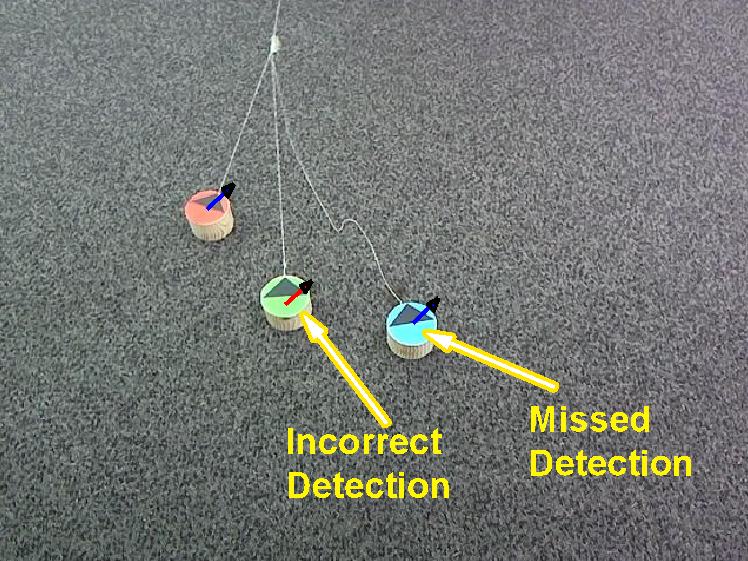
\includegraphics[width=0.5\textwidth]{../Drawings/missedandIncorrectDetData2Ready.pdf}
	\caption{Examples of correct, incorrect and missed arrow orientations respectively}
	\label{fig:missIncorrect}
\end{figure}

\figref{fig:indetect} is an example of one of the shortcomings of the current orientation algorithm. As can be seen in the figure, the bounding box of the robot has been placed around the lower segment of the robot's face. It has completely ignored the arrowhead attached to the robot's upper segment. This is because the upper and lower segments of the robot are separated as there is no 4 or 8 connectivity present between the pixels. The algorithm thus sees the lower segment of the robot as having a larger area and subsequently surrounds that image portion with a bounding box. \\

This creates another problem. The centroid of the bounding box is now found below the center of mass of the robot as seen in the figure. Therefore, when the direction arrow is constructed, the arrow points in the incorrect, and in this case, opposite, direction of the robot's movement.\\ 

  \begin{figure}[h!]
	\centering
		\includegraphics[width=0.5\textwidth]{../Drawings/IncorrectDirectionResults.pdf}
	\caption{Examples of correct, incorrect and missed arrow orientations respectively}
	\label{fig:indetect}
\end{figure}

\subsection{Background Images}
\label{sec:back}
This section analyses the background images produced using the Background Estimation Algorithm detailed in \secref{sec:back}. As can be seen in each of the estimated backgrounds from \figref{fig:backdata1} to \figref{fig:backdata10}, the presence of the robots have caused a slightly blurred effect on each of the images. This is because the corner pixel averaging, detailed in \secref{sec:back}, does not create a perfect representation of the background colour for every pixel that it replaces.\\

Backgrounds with less texture, such as \figref{fig:backdata1}, gave better estimation results. This is because these backgrounds have less colour variation and so the corner pixel averaging technique created a much better representation of the background colour for each pixel.\\

\begin{figure}[h!]
\begin{minipage}[b]{0.5\linewidth}
\includegraphics[scale=0.4]{../Drawings/backdata1.pdf}
\caption{The estimated background image of the first dataset provided for image processing}
\label{fig:backdata1}
\end{minipage}
\hspace{0.5cm}
\begin{minipage}[b]{0.5\linewidth}
\includegraphics[scale=0.3]{../Drawings/backdata2.pdf}
\caption{The estimated background image of the second dataset provided for image processing}
\label{fig:backdata2}
\end{minipage}
\end{figure}


\begin{figure}[h!]
\begin{minipage}[b]{0.5\linewidth}
\includegraphics[scale=0.3]{../Drawings/backdata7.pdf}
\caption{The estimated background image of a new test dataset}
\label{fig:backdata7}
\end{minipage}
\hspace{0.5cm}
\begin{minipage}[b]{0.5\linewidth}
\includegraphics[scale=0.3]{../Drawings/backdata10.pdf}
\caption{The estimated background image of a new test dataset}
\label{fig:backdata10}
\end{minipage}
\end{figure}


%Show an example of results for each stage of detection

\section{Discussion}
\label{sec:discussion}
This section determines the success of the above-mentioned image processing algorithm. In addition, the limitations and problems present in the current design are discussed, as well as future improvements that could be implemented to enhance the algorithm's performance.

\subsection{Success Evaluation}
\label{sec:success}
The image processing algorithm performs particularly well on uniform backgrounds. It is able to detect the robot's in almost every frame and maintains a fairly accurate estimate of the robot's current orientation. Textured backgrounds do interfere with processing each robot's orientation. This is partly due to the normalisation procedure performed on each image frame.\\

The algorithm encounters a problem when a robot leaves the image frame as was the case in dataset 1. Incorrect detections result and incorrect tracks are formed on the image frame. The algorithm also struggles with pixels of high intensity that do not form a part of the robot. If these pixels are the same colour as the robot, they are then incorrectly chosen to represent the robot in the specified image frame.\\

One of the advantages of the algorithm is that it efficiently processes the images at a relatively high speed. This is due to the efficient implementation of the algorithm in Matlab. This is an important feature if the algorithm is to be exposed to larger datasets.

\subsection{Limitations and Problems}
\label{sec:limits}
A prominent problem presented during this project was that of Image-encoding noise \cite{ref:digitalProcessing}. The datasets provided for the project were of a JPEG file type. JPEG images contain compression artefacts which represent data lost due to the compression of the image \cite{ref:digitalProcessing}. These artefacts presented a problem as important image information was lost that could have been useful during image processing. The artefacts themselves were also problematic after the image was normalised, producing pixels of high intensity, which was disruptive to the robot detection process. 

 

\subsection{Future Improvements}
\label{sec:improve}
The \textit{normChannel} Matlab function currently performs contrast stretching on each image. This technique is used to stretch the range of pixel intensity values which ultimately increases the contrast of the image. However, this technique is sensitive to pixel outliers \cite{ref:digitalProcessing}. The algorithm does not currently take this into account. Doing so in a future implementation would result in an improvement in image contrast.\\

The current algorithm used to determine the orientation of the robot could also be improved. An alternative approach would be to calculate the center of mass of the arrowhead situated on the robot. Connecting the robot's center of mass with the arrowhead center of mass may provide an improved estimate of the robot's current orientation.\\

There are also alternative techniques to detecting the robot's in a given image. Once such technique is that of region splitting \cite{ref:digitalProcessing}. This technique treats an image as a single region and iteratively splits the image into sub-regions that share the same, or similar, characteristics. This is achieved using a split-and-merge algorithm. As the process iterates, regions that contain similar characteristics are also merged together. This is an effective way to detect different regions as well as objects in an image.

Another effective method that can be used to detect the robots is edge detection. By taking a Laplacian of a Gaussian (LoG), it is possible to detect the edges of an object \cite{ref:digitalprocessing}. This technique could be applied to the robot images to effectively detect the robot edges.

%Assess the success of the program with regard to:

%1. Report results

%Discuss any
%1. Limitations, problems
%2. Improvements you would make

\section{Code}
\label{sec:code}

\subsection{Read Image Sequences into Matlab}
\label{code:read}

\lstinputlisting{../../myreadfolder.m}

\lstinputlisting{../../myreadimg.m}

\subsection{Background Estimation Functions}
\label{code:background}

\lstinputlisting{../../eraseRegion.m}



\subsection{Detection Algorithm Helper Functions}
\label{code:detection}

\lstinputlisting{../../processChannels.m}

\lstinputlisting{../../myimgblur.m}

\lstinputlisting{../../normalize_rgb.m}

\lstinputlisting{../../normchannel.m}

\lstinputlisting{../../xyhistmax.m}

\lstinputlisting{../../findthresh.m}

\lstinputlisting{../../cliprect.m}

\section{Linking Algorithm Functions}

\lstinputlisting{../../calcBoundingBox.m}


\lstinputlisting{../../calcBoundingBoxCM.m}

\section{Orientation Algorithm Third Party Helper Function}


\lstinputlisting{../../plot_arrow.m}


\subsection{Main Program Code}
\label{code:main}
\lstinputlisting{../../main.m}
%Any downloaded code should be recorded in the report. Does not need to be in the appendix
%Code from course web pages are not needed

\section{Conclusion}
\label{sec:conclusion}
The image processing algorithm developed to detect robots in an image sequence has been detailed. Various techniques such as normalisation, blurring, contrast stretching and histogram smoothing have been implemented in this algorithm. Various sub-algorithms have been defined such as robot detection, linking tracks in successive image frames as well as determining the robot's current orientation. The algorithm was able to maintain near perfect performance in detecting robots. However, if a robot leaves an image frame or there are highly saturated pixels of the same colour as the robot, then the algorithm struggles to detect the robot creating incorrect tracks. An estimated image of the background has been processed. Blurred patches are present on some of the background images, but this can be minimised. Various improvements have also been suggested such as region splitting for detecting the robots as well as finding the center of mass of the arrowhead in order to create a better orientation arrow.

\bibliographystyle{witseie}
\bibliography{bibliography}

% \newpage
%\onecolumn
%\appendix
%\setcounter{table}{0}
%\setcounter{figure}{0}
%\setcounter{subsection}{0}
%\makeatletter \renewcommand{\thefigure}{A.\@arabic\c@figure} \renewcommand{\thetable}{A.\@arabic\c@table} \renewcommand{\thesection}{A.\@arabic\c@section} \makeatother
%\section*{APPENDIX A}
%
%\section{Control Program}
%Add the matlab code to this file...
%\lstinputlisting{codeSnippets.cpp}
 
\end{document}

